\newpage
\section{Sformułowanie problemu i wymagania}

Cel pracy możemy sformułować jako rozwiązanie następujących problemów:
\begin{enumerate}
    \item \textbf{Problem transmisji danych na duże odległości bez infrastruktury zewnętrznej.}
          Czyli jak zapewnić niezawodną wymianę krótkich pakietów między ruchomymi węzłami
          w obszarach bez zasięgu sieci komórkowej, przy skromnym budżecie.
    \item \textbf{Problem optymalizacji zajętości pasma,} co sprowadza się do minimalizacji liczby
          wysyłanych pakietów. Oznacza to opracowanie metod oszczędzania wysyłki lokalizacji GPS,
          np.\ w sytuacjach kiedy węzły są w bezruchu albo daleko od granicy strefy. Warto zauważyć,
          że rozwiązanie tego problemu jest również przydatne ze względu na oszczędzanie baterii
          niewielkich węzłów radiowych.
    \item \textbf{Problem integracji dwóch systemów.} Ponieważ interfejs użytkownika znajduje się
          w smartfonie, konieczne będzie stworzenie integracji aplikacji mobilnej z siecią radiową.
\end{enumerate}

\subsection{Przeznaczenie systemu i charakterystyka użytkownika}

System ma służyć do monitorowania położenia psa myśliwskiego w czasie rzeczywistym w obszarach
pozbawionych pokrycia sieci komórkowej. Użytkownikiem docelowym jest właściciel psa myśliwskiego
przebywający na działce lub w terenie otwartym - osoba niekoniecznie posiadająca wiedzę techniczną
z zakresu sieci radiowych czy programowania. Z charakterystyki użytkownika wynikają następujące
założenia projektowe:
\begin{itemize}
    \item interfejs aplikacji mobilnej musi być przejrzysty i niewymagający konfiguracji
          przy każdym uruchomieniu,
    \item konfiguracja sprzętu radiowego powinna być jednorazowa lub niewymagana oraz nie powinna
          wymagać interwencji użytkownika w trakcie normalnej eksploatacji,
    \item powiadomienia o przekroczeniu strefy muszą być jednoznaczne i natychmiastowe, również
          gdy aplikacja jest zminimalizowana albo telefon ma wygaszony ekran.
\end{itemize}

Typowy scenariusz użycia wygląda następująco: właściciel przebywa na działce, pies porusza się
swobodnie po terenie. Właściciel uruchamia aplikację, obserwuje pozycję psa na mapie i otrzymuje
alarm wibracyjny lub dźwiękowy w momencie, gdy pies oddali się poza zdefiniowaną strefę
bezpieczeństwa.

\subsection{Wymagania funkcjonalne}

Zdefiniowałem wymagania funkcjonalne z podziałem na fazy projektu.

\subsubsection{Faza 1 - Wizualizacja pozycji}
\begin{itemize}
    \item System musi odbierać dane o pozycji GPS węzła mobilnego.
    \item Aplikacja musi wyświetlać pozycję wszystkich aktywnych węzłów na mapie w czasie
          rzeczywistym.
    \item Aplikacja powinna przechowywać historię pozycji węzłów z bieżącej sesji.
\end{itemize}

\subsubsection{Faza 2 - Geofencing}
\begin{itemize}
    \item Użytkownik musi mieć możliwość zdefiniowania strefy bezpieczeństwa w postaci wielokąta
          na mapie.
    \item System musi wykrywać przekroczenie granicy strefy przez węzeł mobilny.
    \item Aplikacja musi powiadamiać użytkownika o przekroczeniu strefy również gdy działa w tle.
    \item Zdefiniowane strefy muszą być przechowywane między sesjami aplikacji.
    \item Użytkownik powinien mieć możliwość definiowania wielu stref jednocześnie.
\end{itemize}

\subsubsection{Faza 3 - Rozszerzenia}
\begin{itemize}
    \item System powinien różnicować częstotliwość wysyłania pozycji w zależności od stanu ruchu
          węzła.
    \item Aplikacja powinna umożliwiać przypisanie nazwy i ikony do każdego węzła.
\end{itemize}

\subsection{Wymagania parametryczne}

Dodatkowo zebrałem wymagania parametryczne opisujące mierzalne cechy części składowych systemu.

\subsubsection{Parametry sieci radiowej}
\begin{itemize}
    \item Węzły powinny komunikować się na minimalną odległość 2 kilometrów w terenie polnym
          i częściowo zalesionym, z dostarczalnością pakietów na poziomie minimum 90\%.
          Zadany zasięg pracy wynika z praktyki, która wskazuje, że mniej więcej taka odległość
          jest wystarczająca do prowadzenia poszukiwania psa w wypadku ucieczki/pogoni za zwierzyną.
    \item Opóźnienie dostarczania pakietów w sieci nie powinno przekraczać 3 sekund. Ta wartość
          podyktowana jest koniecznością reakcji w przypadku opuszczenia strefy przez psa.
          Zbyt duże opóźnienie mogłoby spowodować utratę cennego czasu reakcji.
\end{itemize}

\subsubsection{Parametry węzła mobilnego (obroża)}
\begin{itemize}
    \item Węzeł mobilny powinien być możliwie mały i lekki, aby zapewnić możliwość przymocowania
          do obroży średniej wielkości psa (ok.\ 20~kg).
    \item Powinien być odporny na warunki atmosferyczne, zachlapania wodą oraz uszkodzenia
          mechaniczne.
\end{itemize}

\subsubsection{Parametry aplikacji mobilnej}
\begin{itemize}
    \item Aplikacja powinna działać na platformie Android w wersji 8.0 lub nowszej.
    \item Aplikacja musi mieć możliwość działania w tle.
\end{itemize}

\subsection{Przegląd istniejących rozwiązań}

Środowisko myśliwskie zna wiele rozwiązań na utrzymywanie psów w ściśle zdefiniowanych obszarach.
Rozważając jedynie elektroniczne rozwiązania, przedstawię tutaj jedynie te najlepiej dopracowane.

\subsubsection{Dogtra Pathfinder 2}

Jest to jeden z najbardziej zaawansowanych produktów z tej dziedziny. Zestaw składa się
z odbiornika, który łączy się z telefonem przez Bluetooth, oraz jednego lub więcej (maksymalnie 21)
nadajników umieszczonych na obrożach elektronicznych. Urządzenia łączą się ze sobą po falach
radiowych. Odbiornik zarówno przekazuje dane z nadajników, jak też daje możliwość użycia przycisku,
który może być zaprogramowany do wzbudzania impulsów elektrycznych w obroży, emitowania światła,
dźwięku albo wibracji w nadajnikach. Aplikacja \textit{PATHFINDER2} łącząca się przez Bluetooth
z odbiornikiem służy do wyświetlania dokładnej pozycji wszystkich skonfigurowanych nadajników,
podglądania ich stanu, sprawdzania naładowania baterii nadajników oraz statusu połączenia z GPS.
Pozatym aplikacja umożliwia nagrywanie lokalizacji w sesje do późniejszego odtworzenia, nawigację
na Mapach Google, pomiary odległości oraz sterowanie modułami na nadajnikach (wibracja, dźwięk,
światło, impuls elektryczny).

Ciekawą funkcją jest możliwość definiowania różnego rodzaju ,,E-Ogrodzeń''. Firma Dogtra opracowała
trzy rodzaje:
\begin{enumerate}
    \item \textbf{Mobile-Fence} - ogrodzenie poruszające się w oparciu o lokalizację smartfona
          i wysyłające powiadomienia.
    \item \textbf{Geo-Fence} - konfiguracja statycznego ogrodzenia wysyłającego powiadomienia.
    \item \textbf{E-Fence} - statyczna konfiguracja ogrodzenia wysyłająca psu automatyczną
          korektę i powiadomienie.\footnote{Dogtra Pathfinder 2 - instrukcja obsługi, s.~26.
          Dostępna pod adresem:
          \url{https://i00.eu/file/403/15309-manualplpathfinder2.pdf}}
\end{enumerate}

Producent deklaruje następujące parametry pracy:
\begin{itemize}
    \item zasięg do 9 mil (ok.\ 14~484~m),
    \item aktualizacje pozycji co 2 sekundy,
    \item użytkowanie bez dodatkowych opłat abonamentowych.
\end{itemize}

% TODO: Skopiuj pliki dogtra.jpg oraz dogtraremote.png do katalogu img/
%       Plik dogtraremote.webp wymaga konwersji do formatu PNG przed użyciem.
\begin{figure}[!h]
    \caption{Dogtra Pathfinder 2 - odbiornik}
    \label{fig:dogtra-receiver}
    \centering
    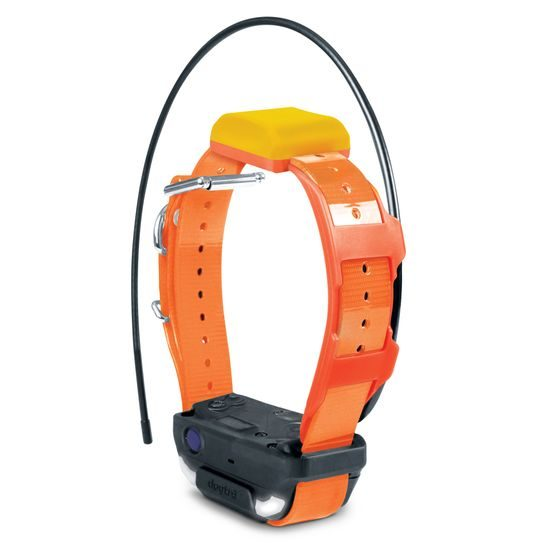
\includegraphics[width=0.5\linewidth]{dogtra.jpg}
\end{figure}

\begin{figure}[!h]
    \caption{Dogtra Pathfinder 2 - pilot zdalnego sterowania}
    \label{fig:dogtra-remote}
    \centering
    
\includegraphics[width=0.5\linewidth]{dogtraremote.png}
\end{figure}

\subsubsection{Dogtrace DOG GPS X25}

Jedynie nieznacznie różnym podejściem wykazała się firma Dogtrace, która w swoim rozwiązaniu
zdecydowała się zrezygnować z konieczności użycia smartfona. X25 składa się z identycznego
funkcjonalnie nadajnika oraz znacznie rozbudowanego odbiornika - wielkości mniejszego smartfona -
który na wbudowanym wyświetlaczu LCD pokazuje kierunek i odległość do nadajnika. Czeska firma
udostępniła lepszej jakości informacje o funkcjonowaniu swojego produktu. Z oferty na stronie
internetowej\footnote{\url{https://www.obroza-elektryczna.pl/dogtrace-dog-gps-x25}} dowiadujemy
się, że:
\begin{itemize}
    \item możliwe jest śledzenie do 19 psów jednocześnie,
    \item bateria nadajnika i odbiornika powinna wystarczyć na ponad 40 godzin pracy (Li-Pol
          1900~mAh),
    \item pozycjonowanie modułów zapewnia skorzystanie z kilku systemów: GPS, GALILEO, GLONASS,
          a nadajnik z odbiornikiem łączą się po LoRa,
    \item deklarowany zasięg to 20~km dla komunikacji ,,w linii wzroku'',
    \item pełna zanurzalność nadajnika i odbiornika.
\end{itemize}

Dodatkowo dostępne są funkcje takie jak: KOMPAS (kierunek na północ magnetyczną), BEEPER
(wykrywanie ruchu lub bezruchu psa), FENCE (okrągły płot - akustyczna granica wyznaczająca
przestrzeń dla psa), WAYPOINT (możliwość zapisania 4 współrzędnych GPS odbiornika i nawigacja
do tych punktów), tryb CAR (umożliwiający korzystanie z odbiornika w pojeździe) oraz sygnał
dźwiękowy zastępujący gwizdek (3 różne dźwięki do wyboru).

% TODO: Skopiuj plik Dogtrace.png do katalogu img/
\begin{figure}[!h]
    \caption{Dogtrace DOG GPS X25}
    \label{fig:dogtrace-x25}
    \centering
    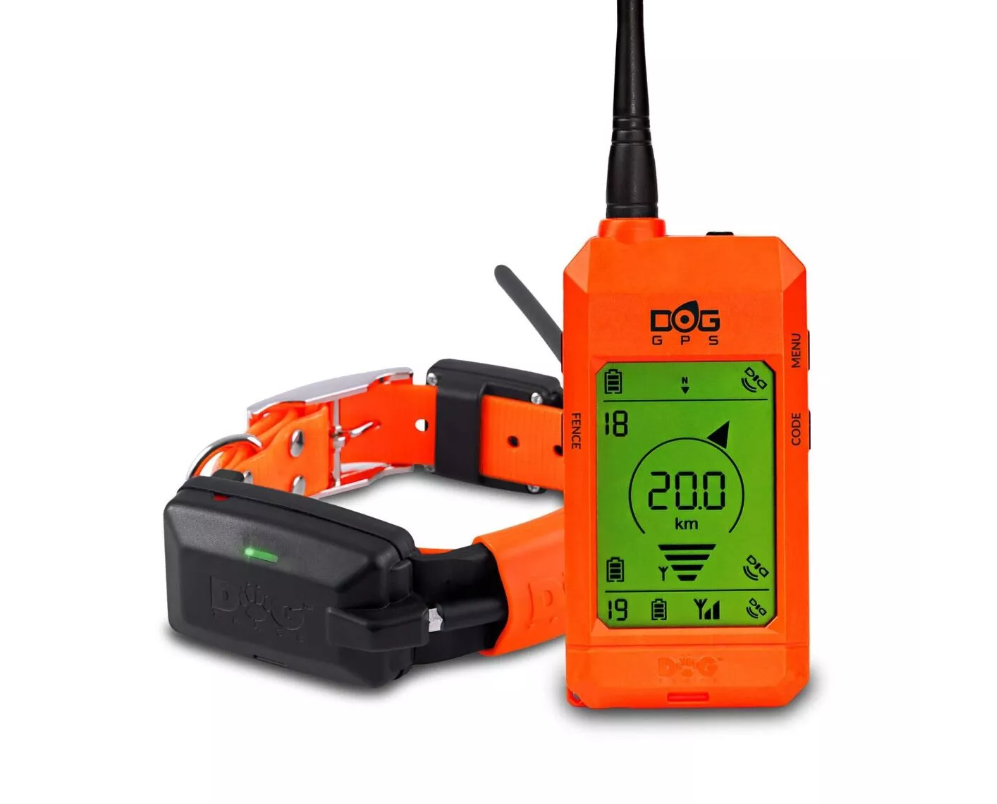
\includegraphics[width=0.5\linewidth]{Dogtrace.png}
\end{figure}
